\graphicspath{ {/home/jefferson/Modelamento/} }
\chapter{Resultados Parciais}
No cap\'itulo anterior foram abordados os principais aspectos sobre o problema de planejamento, a teoria utilizada e o
aspecto do algoritmo tamb\'em foi discutido. Nesse cap\'itulo seram abordados os resultados parciais da pesquisa.
A simula\c c\~ao  foi constitu\'ida para um sistema hidrot\'ermico de duas usinas hidrel\'etricas em cascata
com duas termel\'etricas associadas considerando-se dois cen\'arios com probabilidade $p$ e $1-p$ respectivamente.
O sistema foi configurado de tal forma a garantir a demanda da regi\~ao dada por,
\symbl{$\pho_i, i = 1, 2 \dots$}{\'Indice de produtibilidade}
\abbrev{H1}{Hidrel\'etrica 1}
\abbrev{H2}{Hidrel\'etrica 2}
\abbrev{T1}{Termel\'etrica 1}
\abbrev{T2}{Termel\'etrica 2}
\abbrev{VTH1}{Volume Turbinado de H1}
\abbrev{VTH2}{Volume Turbinado de H2}
\abbrev{VI}{Volume Inicial}
\abbrev{VV}{Volume Vertido}
\abbrev{G1}{Produ\c c\~ao da Termel\'etrica T1}
\abbrev{G2}{Produ\c c\~ao da Termel\'etrica T2}
\abbrev{VIC}{Volume Incremental}
\symbl{Gmax}{Produ\c c\~ao M\'axima da term\'eletricas}
\begin{align*}
  \displaystyle{\rho}_1*VTH1 + {\rho}_2*VTH2 + G1 + G2 = DEMANDA,
\end{align*}
onde:
\begin{itemize}
	\item $H_1$ e $H_2$ representam as hidrel\'etricas associadas ao sistema;
	\item $G_1$ e $G_2$ representam as termel\'etricas associadas ao sistema;
	\item $\rho_1$ e $\rho_2$ s\~ao os \'indices de produtibilidade das usinas H1 e H2;
	\item $VTH1$ e $VTH$  os volumes turbinados das hidrel\'etricas associadas.
\end{itemize}
O sistema deve preservar o balan\c co hidr\'ico dada por,
{\setlength{\belowdisplayskip}{-4pt}
\begin{align*}
  \displaystyle Vt = VI + VIC - \left( VT + VV \right), 
\end{align*}}
onde : 
\begin{itemize}
	\item $V(t)$ representar o volume em qualquer instante de tempo;
	\item $VI$  volume inicial;
	\item $VIC$ volume incremental;
	\item $VV$ volume vertido
\end{itemize}
Por quest\~oes relacionadas ao custo e ao ambiente a gera\c c\~ao das termel\'etricas devem respeitar uma toler\^ancia de
gera\c c\~ao dada por:
\begin{align*}
	G_1 + G_2 \leq G_{max}
\end{align*}
onde $G_{max}$ representar a produ\c c\~ao m\'axima das termel\'etricas associadas aos sistema. O n\'ivel de
produtibilidade adotado na simula\c c\~ao ser\'a nomeado por $\rho$. 
Os resultados para a
simula\c c\~ao considerando as probabilidades do cen\'arios 1 e 2 seram denominados  por $p$ e $ 1 -
p$ respectivamente. A seguir os resultados das simula\c c\~oes.

\begin{figure}[!ht]
	\centering
	\subfigure[$\rho = 1,0$.]{
		\label{gf1a}
		\includegraphics[width=6cm,height=5cm]{prob.0.1/simulacao.1.0/simula.pdf}
	}
	\subfigure[$\rho = 1,4$.]{
		\label{gf1b}
		\includegraphics[width=6cm,height=5cm]{prob.0.1/simulacao.1.4/simula.pdf}
	}
	\subfigure[$\rho = 1,5$.]{
		\label{gf1c}
		\includegraphics[width=6cm,height=5cm]{prob.0.1/simulacao.1.5/simula.pdf}
	}
	\subfigure[$\rho = 1,6$.]{
		\label{gf1d}
		\includegraphics[width=6cm,height=5cm]{prob.0.1/simulacao.1.6/simula.pdf}
	}
	\subfigure[$\rho = 1,8$.]{
		\label{gf1e}
		\includegraphics[width=6cm,height=5cm]{prob.0.1/simulacao.1.8/simula.pdf}
	}
	\subfigure[$\rho = 2,0$.]{
		\label{gf1f}
		\includegraphics[width=6cm,height=5cm]{prob.0.1/simulacao.2.0/simula.pdf}
	}
	\caption{Simula\c c\~ao para cen\'arios de probabilidade $p = 0.1$ e $1 - p = 0.9$.}
	\label{gf1}
\end{figure}

\begin{figure}
	\centering
	\subfigure[Custo para $\rho = 1,0.$]{
		\includegraphics[width=7cm,height=7cm]{prob.0.1/simulacao.1.0/custo.pdf}
	}
	\subfigure[Custo para $\rho = 1,4.$]{
		\includegraphics[width=7cm,height=7cm]{prob.0.1/simulacao.1.4/custo.pdf}
	}
	\subfigure[Custo para $\rho = 1,5.$]{
		\includegraphics[width=7cm,height=7cm]{prob.0.1/simulacao.1.5/custo.pdf}
	}
	\subfigure[Custo para $\rho = 1,6.$]{
		\includegraphics[width=7cm,height=7cm]{prob.0.1/simulacao.1.6/custo.pdf}
	}
	\subfigure[Custo para $\rho = 1,8.$]{
		\includegraphics[width=7cm,height=7cm]{prob.0.1/simulacao.1.8/custo.pdf}
	}
	\subfigure[Custo para $\rho = 2,0.$]{
		\includegraphics[width=7cm,height=7cm]{prob.0.1/simulacao.2.0/custo.pdf}
	}
	\caption{Simula\c c\~ao da curva de custo esperado $p = 0.1$ e $1 - p = 0.9$.}
	\label{cu1}
\end{figure}

\begin{figure}[!ht]
	\centering
	\subfigure[$\rho = 1,0$.]{
		\label{gf2a}
		\includegraphics[width=7cm,height=7cm]{prob.0.2/simulacao.1.0/simula.pdf}
	}
	\subfigure[$\rho = 1,4$.]{
		\label{gf2b}
		\includegraphics[width=7cm,height=7cm]{prob.0.2/simulacao.1.4/simula.pdf}
	}
	\subfigure[$\rho = 1,5$.]{
		\label{gf2c}
		\includegraphics[width=7cm,height=7cm]{prob.0.2/simulacao.1.5/simula.pdf}
	}
	\subfigure[$\rho = 1,6$.]{
		\label{gf2d}
		\includegraphics[width=7cm,height=7cm]{prob.0.2/simulacao.1.6/simula.pdf}
	}
	\subfigure[$\rho = 1,8$.]{
		\label{gf2e}
		\includegraphics[width=7cm,height=7cm]{prob.0.2/simulacao.1.8/simula.pdf}
	}
	\subfigure[$\rho = 2,0$.]{
		\label{gf2f}
		\includegraphics[width=6cm,height=5cm]{prob.0.2/simulacao.2.0/simula.pdf}
	}
	\caption{Simula\c c\~ao para cen\'arios de probabilidade $p = 0.2$ e $1 - p = 0.8$.}
	\label{gf2}
\end{figure}

\begin{figure}[!ht]
	\centering
	\subfigure[Custo para $\rho = 1,0.$]{
		\includegraphics[width=7cm,height=7cm]{prob.0.2/simulacao.1.0/custo.pdf}
	}
	\subfigure[Custo para $\rho = 1,4.$]{
		\includegraphics[width=7cm,height=7cm]{prob.0.2/simulacao.1.4/custo.pdf}
	}
	\subfigure[Custo para $\rho = 1,5.$]{
		\includegraphics[width=7cm,height=7cm]{prob.0.2/simulacao.1.5/custo.pdf}
	}
	\subfigure[Custo para $\rho = 1,6.$]{
		\includegraphics[width=7cm,height=7cm]{prob.0.2/simulacao.1.6/custo.pdf}
	}
	\subfigure[Custo para $\rho = 1,8.$]{
		\includegraphics[width=7cm,height=7cm]{prob.0.2/simulacao.1.8/custo.pdf}
	}
	\subfigure[Custo para $\rho = 2,0.$]{
		\includegraphics[width=7cm,height=7cm]{prob.0.2/simulacao.2.0/custo.pdf}
	}
	\caption{Simula\c c\~ao da curva de custo esperado $p = 0.2$ e $1 - p = 0.8$.}
	\label{cu2}
\end{figure}

\begin{figure}[!ht]
	\centering
	\subfigure[$\rho = 1,0$.]{
		\label{gf3a}
		\includegraphics[width=7cm,height=7cm]{prob.0.5/simulacao.1.0/simula.pdf}
	}
	\subfigure[$\rho = 1,4$.]{
		\label{gf3b}
		\includegraphics[width=7cm,height=7cm]{prob.0.5/simulacao.1.4/simula.pdf}
	}
	\subfigure[$\rho = 1,5$.]{
		\label{gf3c}
		\includegraphics[width=7cm,height=7cm]{prob.0.5/simulacao.1.5/simula.pdf}
	}
	\subfigure[$\rho = 1,6$.]{
		\label{gf3d}
		\includegraphics[width=7cm,height=7cm]{prob.0.5/simulacao.1.6/simula.pdf}
	}
	\subfigure[$\rho = 1,8$.]{
		\label{gf3e}
		\includegraphics[width=7cm,height=7cm]{prob.0.5/simulacao.1.8/simula.pdf}
	}
	\subfigure[$\rho = 2,0$.]{
		\label{gf3f}
		\includegraphics[width=6cm,height=5cm]{prob.0.5/simulacao.2.0/simula.pdf}
	}
	\caption{Simula\c c\~ao para cen\'arios de probabilidade $p = 0.5$ e $1 - p = 0.5$.}
	\label{gf3}
\end{figure}

\begin{figure}[!ht]
	\centering
	\subfigure[Custo para $\rho = 1,0.$]{
		\includegraphics[width=7cm,height=7cm]{prob.0.5/simulacao.1.0/custo.pdf}
	}
	\subfigure[Custo para $\rho = 1,4.$]{
		\includegraphics[width=7cm,height=7cm]{prob.0.5/simulacao.1.4/custo.pdf}
	}
	\subfigure[Custo para $\rho = 1,5.$]{
		\includegraphics[width=7cm,height=7cm]{prob.0.5/simulacao.1.5/custo.pdf}
	}
	\subfigure[Custo para $\rho = 1,6.$]{
		\includegraphics[width=7cm,height=7cm]{prob.0.5/simulacao.1.6/custo.pdf}
	}
	\subfigure[Custo para $\rho = 1,8.$]{
		\includegraphics[width=7cm,height=7cm]{prob.0.5/simulacao.1.8/custo.pdf}
	}
	\subfigure[Custo para $\rho = 2,0.$]{
		\includegraphics[width=7cm,height=7cm]{prob.0.2/simulacao.2.0/custo.pdf}
	}
	\caption{Simula\c c\~ao da curva de custo esperado $p = 0.5$ e $1 - p = 0.5$.}
	\label{cu3}
\end{figure}

\begin{figure}[!ht]
	\centering
	\subfigure[$\rho = 1,0$.]{
		\label{gf4a}
		\includegraphics[width=7cm,height=7cm]{prob.0.7/simulacao.1.0/simula.pdf}
	}
	\subfigure[$\rho = 1,4$.]{
		\label{gf4b}
		\includegraphics[width=7cm,height=7cm]{prob.0.7/simulacao.1.4/simula.pdf}
	}
	\subfigure[$\rho = 1,5$.]{
		\label{gf4c}
		\includegraphics[width=7cm,height=7cm]{prob.0.7/simulacao.1.5/simula.pdf}
	}
	\subfigure[$\rho = 1,6$.]{
		\label{gf4d}
		\includegraphics[width=7cm,height=7cm]{prob.0.7/simulacao.1.6/simula.pdf}
	}
	\subfigure[$\rho = 1,8$.]{
		\label{gf4e}
		\includegraphics[width=6cm,height=7cm]{prob.0.7/simulacao.1.8/simula.pdf}
	}
	\subfigure[$\rho = 2,0$.]{
		\label{gf4f}
		\includegraphics[width=7cm,height=7cm]{prob.0.7/simulacao.2.0/simula.pdf}
	}
	\caption{Simula\c c\~ao para cen\'arios de probabilidade $p = 0.7$ e $1 - p = 0.3$.}
	\label{gf4}
\end{figure}

\begin{figure}[!ht]
	\centering
	\subfigure[Custo para $\rho = 1,0.$]{
		\includegraphics[width=7cm,height=7cm]{prob.0.7/simulacao.1.0/custo.pdf}
	}
	\subfigure[Custo para $\rho = 1,4.$]{
		\includegraphics[width=7cm,height=7cm]{prob.0.7/simulacao.1.4/custo.pdf}
	}
	\subfigure[Custo para $\rho = 1,5.$]{
		\includegraphics[width=7cm,height=7cm]{prob.0.7/simulacao.1.5/custo.pdf}
	}
	\subfigure[Custo para $\rho = 1,6.$]{
		\includegraphics[width=7cm,height=7cm]{prob.0.7/simulacao.1.6/custo.pdf}
	}
	\subfigure[Custo para $\rho = 1,8.$]{
		\includegraphics[width=7cm,height=7cm]{prob.0.7/simulacao.1.8/custo.pdf}
	}
	\subfigure[Custo para $\rho = 2,0.$]{
		\includegraphics[width=7cm,height=7cm]{prob.0.7/simulacao.2.0/custo.pdf}
	}
	\caption{Simula\c c\~ao da curva de custo esperado $p = 0.7$ e $1 - p = 0.3$.}
	\label{cu4}
\end{figure}

\begin{figure}[!ht]
	\centering
	\subfigure[$\rho = 1,0$.]{
		\label{gf5a}
		\includegraphics[width=7cm,height=7cm]{prob.1.0/simulacao.1.0/simula.pdf}
	}
	\subfigure[$\rho = 1,4$.]{
		\label{gf5b}
		\includegraphics[width=7cm,height=7cm]{prob.1.0/simulacao.1.4/simula.pdf}
	}
	\subfigure[$\rho = 1,5$.]{
		\label{gf5c}
		\includegraphics[width=7cm,height=7cm]{prob.1.0/simulacao.1.5/simula.pdf}
	}
	\subfigure[$\rho = 1,6$.]{
		\label{gf5d}
		\includegraphics[width=7cm,height=7cm]{prob.1.0/simulacao.1.6/simula.pdf}
	}
	\subfigure[$\rho = 1,8$.]{
		\label{gf5e}
		\includegraphics[width=7cm,height=7cm]{prob.1.0/simulacao.1.8/simula.pdf}
	}
	\subfigure[$\rho = 2,0$.]{
		\label{gf5f}
		\includegraphics[width=7cm,height=7cm]{prob.1.0/simulacao.2.0/simula.pdf}
	}
	\caption{Simula\c c\~ao para cen\'arios de probabilidade $p = 1.0$ e $1 - p = 0.0$.}
	\label{gf5}
\end{figure}

\begin{figure}[!ht]
	\centering
	\subfigure[Custo para $\rho = 1,0.$]{
		\includegraphics[width=7cm,height=7cm]{prob.1.0/simulacao.1.0/custo.pdf}
	}
	\subfigure[Custo para $\rho = 1,4.$]{
		\includegraphics[width=7cm,height=7cm]{prob.1.0/simulacao.1.4/custo.pdf}
	}
	\subfigure[Custo para $\rho = 1,5.$]{
		\includegraphics[width=7cm,height=7cm]{prob.1.0/simulacao.1.5/custo.pdf}
	}
	\subfigure[Custo para $\rho = 1,6.$]{
		\includegraphics[width=7cm,height=7cm]{prob.1.0/simulacao.1.6/custo.pdf}
	}
	\subfigure[Custo para $\rho = 1,8.$]{
		\includegraphics[width=7cm,height=7cm]{prob.1.0/simulacao.1.8/custo.pdf}
	}
	\subfigure[Custo para $\rho = 2,0.$]{
		\includegraphics[width=7cm,height=7cm]{prob.1.0/simulacao.2.0/custo.pdf}
	}
	\caption{Simula\c c\~ao da curva de custo esperado $p = 1.0$ e $1 - p = 0.0$.}
	\label{cu5}
\end{figure}
\clearpage
A figura (\ref{gf1}) \'e constitu\'ida por configura\c c\~oes distintas de planejamento que est\~ao associados a produtibilidade das usinas
hidrel\'etricas. Nas figuras (\ref{gf1a}) e (\ref{gf1b}) nota-se uma gera\c c\~ao predominantemente da hidrel\'etrica H1
para um intervalo inicial de demanda.
Entretanto, a medida que o aumento de demanda torna-se significativo para o sistema ocorre a ativa\c c\~ao da Hidrel\'etrica H2
e da termel\'etrica T1. Observa-se que ocorre um aumento da gera\c c\~ao de H2 e a gera\c c\~ao de T1 permanece constante no per\'iodo de estudo.
As figuras (\ref{gf1b}) e (\ref{gf1c}) possuem como principal aspecto relevante a vasta utiliza\c c\~ao
da gera\c c\~ao de H2 para essa configura\c c\~ao de despacho. Por fim, as figuras (\ref{gf1e}) e (\ref{gf1f}) possuem ampla gera\c c\~ao de H2.
Contudo, sua principal caracter\'istica \'e ativa\c c\~ao posterior de T1 em compara\c c\~ao aos outros casos.
Em resumo, de acordo com a figura (\ref{gf1}), a medida que ocorre uma altera\c c\~ao na produtibilidade de H1
e o sistema sofre uma aumento na demanda, o arranjo da gera\c c\~ao \'e alterado. Nota-se comportamento semelhante
observando-se o despaco hidrot\'ermico nas figuras (\ref{gf2}),(\ref{gf3}),(\ref{gf4}) e (\ref{gf5}). 

Conforme descrito em figura (\ref{cu1}), as configura\c c\~oes de produtibilidade para aumento da demanda tiveram um
impacto consider\'avel no valor de custo. De fato, percebe-se uma suaviza\c c\~ao da curva do valor \'otimo para o custo
associado ao sistema. No primeiro momento ocorre um crescimento sim\'etrico em ambos os casos descritos na figura
(\ref{gf1}). Por\'em, a medida que ocorre uma crescimento na demanda. Em determinada ocasi\~ao observa-se uma ruptura na
sim\'etria da curva ocorrendo um aumento do custo, posteriormente, o equil\'ibrio \'e atingido. Nota-se que as mudan\c
cas ocorridas nos cen\'arios de probabilidades distintos de maneira geral n\~ao modificaram as curva de custo esperado
descrito nas figuras (\ref{cu1}),(\ref{cu2}),(\ref{cu3}),(\ref{cu4}) e (\ref{cu5}).

A configura\c c\~ao da
produtibilidade considerada de maior import\^ancia para o despacho hidrot\'ermico com base nas simula\c c\~oes \'e a
encontrada nas figuras
(\ref{gf1e}) e (\ref{gf1f}). Pois, ocorre uma adapta\c c\~ao favor\'avel do sistema pelo
aspecto do custo, uma vez que pela suaviza\c c\~ao ocorrida evita-se aumentos inesperados. O segundo ponto  \'e a
relev\^ancia ambiental associada com o uso das termel\'etricas. Visto que, a termel\'etrica T1 \'e ativada em um
per\'iodo posterior em rela\c c\~ao as outras configura\c c\~oes. Desta forma, o sistema utilizando-se da configura\c
c\~ao nas figuras (\ref{gf1e}),(\ref{gf1f}),(\ref{gf2e}),(\ref{gf2f}),(\ref{gf3e}),
(\ref{gf3f}),(\ref{gf4e}),(\ref{gf4f}),(\ref{gf5e}),(\ref{gf5f})
manteve-se em condi\c c\~oes de adapta\c c\~oes para o aumento na demanda. Vale salientar,
que a ruptura observada na figura (\ref{gf1}) e nas outras simula\c c\~oes deve-se em todos casos deve-se ao \^onus da ativa\c c\~ao de T1.
Para a presente
an\'alise considerou-se v\'arios outros cen\'arios com probabilidades distintas. Contudo, pelos resultados no aspecto
geral serem semelhantes esses cen\'arios n\~ao foram descritos no presente trabalho. Por fim, a figura(\ref{despacho}) a seguir descreve
de forma b\'asica as configura\c c\~oes encontradas. A configura\c c\~ao satisfat\'oria \'e a segunda.
\newpage
\begin{figure}[!h]
    \centering
    \resizebox{0.8\textwidth}{!}{%
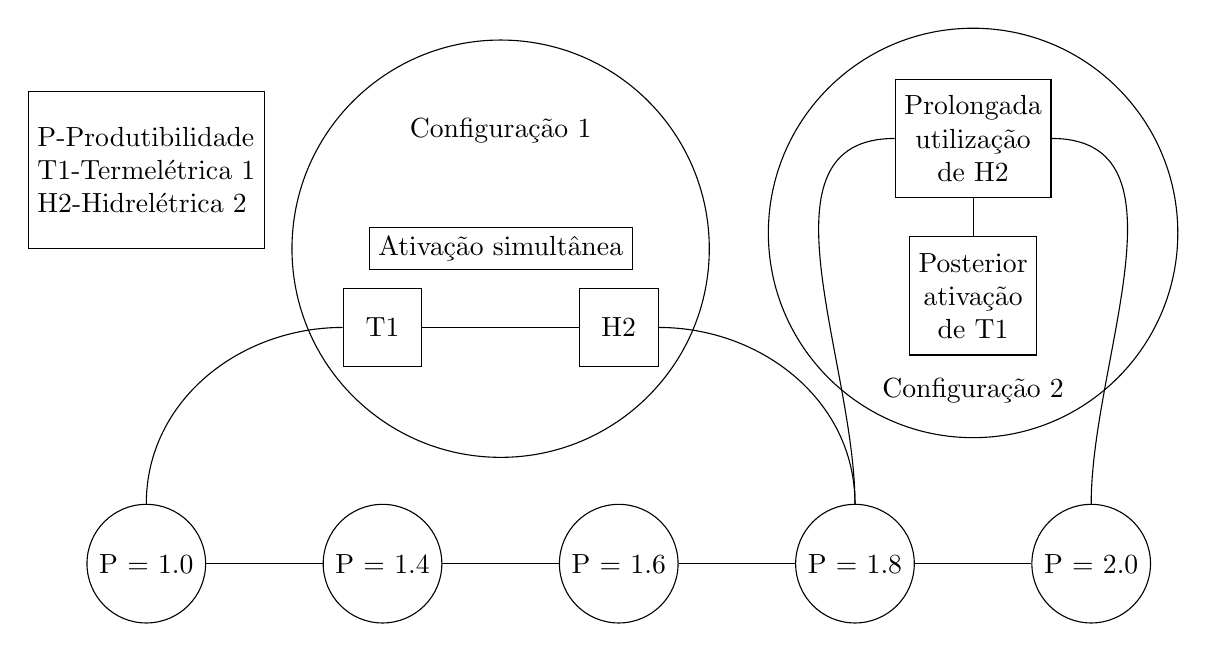
\begin{tikzpicture}
  \draw node[draw, circle] (p10) at (1,1) {P = 1.0};
  \draw node[draw, circle] (p14) at (4,1) {P = 1.4};
  \draw node[draw, circle] (p16) at (7,1) {P = 1.6};
  \draw node[draw, circle] (p18) at (10,1) {P = 1.8};
  \draw node[draw, circle] (p20) at (13,1) {P = 2.0};
  \draw [draw] (p10) to [out=0,in=180] (p14);
  \draw [draw] (p14) to [out=0,in=180] (p16);
  \draw [draw] (p16) to [out=0,in=180] (p18);
  \draw [draw] (p18) to [out=0,in=180] (p20);
  \node [draw](S) at (5.5,5.0) {Ativa\c c\~ao simult\^anea};
  \node [draw, circle, minimum size=5.3cm](c1) at (5.5,5.0) {};
  \node [draw, minimum size=1.0cm] (t1) at (4,4) {T1};
  \node [draw, minimum size=1.0cm] (h2) at (7,4) {H2}; 
  \draw [draw] (t1) to [out=0,in=180] (h2); 
  \draw [draw] (p10) to [out=90,in=180] (t1); 
  \draw [draw] (p18) to [out=90,in=0] (h2); 
  \draw node [] at (5.5, 6.5){Configura\c c\~ao 1};
  \draw node[align=center,draw, minimum size=1.5cm](h) at (11.5,6.4) {Prolongada\\ utiliza\c c\~ao \\de H2};  
  \draw [draw] (p18) to [out=90,in=180] (h);
  \draw [draw] (p20) to [out=90,in=0] (h);
  \draw node[align=center,draw, minimum size=1.5cm](t) at (11.5,4.4) {Posterior\\ ativa\c c\~ao \\de T1};  
  \draw [draw] (h) to [out=270,in=90] (t);
  \node [draw, circle, minimum size=5.2cm](c1) at (11.5,5.2) {};
  \draw node [] at (11.5, 3.2){Configura\c c\~ao 2};
  \node [draw,align=justify, minimum size=2cm]() at (1.0,6.0) {P-Produtibilidade\\
  T1-Termel\'etrica 1\\H2-Hidrel\'etrica 2 };
\end{tikzpicture}}

    \caption{Configura\c c\~oes para o despacho hidrot\'ermico.}
	\label{despacho}
\end{figure}

\section{Considera\c c\~oes finais}
Nesse cap\'itulo foram abordados os resultados parciais da pesquisa. Nota-se que a varia\c c\~ao de produtibilidade
modificou a configura\c c\~ao do sistema. Contudo, pelos \'indices de produtibilidade dos resultados abordados nesse
cap\'itulo percebe-se que
o sistema para uma configura\c c\~ao favor\'avel necessita de um alto n\'ivel de produtibilidade. Como \'indice de
produtibilidade \'e uma caracter\'istica da regi\~ao de localiza\c c\~ao da hidrel\'etrica a depend\^encia desse
\'indice ainda n\~ao \'e o ideal
para o planejamento. 

%\section{Lista de tabelas das simula\c c\~oes}
%\begin{table}[!h]
%\input{../../prob.0.1/simulacao.1.1/tabela0.11.1.dat}
%	\caption{Dados da simula\c c\~ao do despacho para $p = 0.1$ e $1 - p = 0.9$}
%\end{table}

